% ------------------------------------------------------------------------------
% TYPO3 CMS 6.2 LTS - What's New - Chapter "Backend Changes" (English Version)
%
% @author	Michael Schams <schams.net>
% @license	Creative Commons BY-NC-SA 3.0
% @link		http://typo3.org/download/release-notes/whats-new/
% @language	English
% ------------------------------------------------------------------------------
% Chapter: Backend Changes
% ------------------------------------------------------------------------------

\section{Backend Changes}
\begin{frame}[fragile]
	\frametitle{Backend Changes}

	\begin{center}\huge{Chapter 3:}\end{center}
	\begin{center}\huge{\color{typo3darkgrey}\textbf{Backend Changes}}\end{center}

\end{frame}

% ------------------------------------------------------------------------------
% Autofocus
% ------------------------------------------------------------------------------
% http://forge.typo3.org/issues/49228

\begin{frame}[fragile]
	\frametitle{Backend Changes}
	\framesubtitle{Backend Login}

 	\begin{itemize}
		\item Autofocus on username field in the backend login form\newline
			(HTML5 attribute: \texttt{autofocus="autofocus"})
	\end{itemize}

	\begin{figure}
		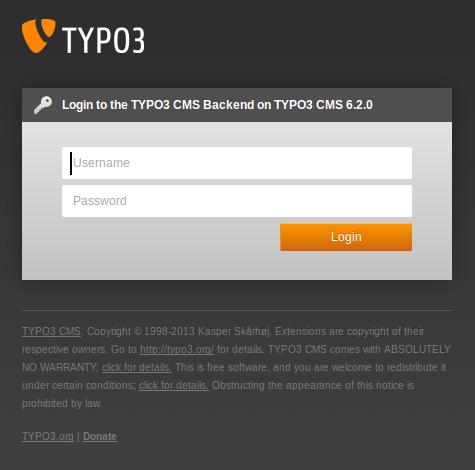
\includegraphics[width=0.4\linewidth]{Images/BackendChanges/BackendLogin.png}
	\end{figure}

\end{frame}

% ------------------------------------------------------------------------------
% Visual Appearance
% ------------------------------------------------------------------------------
% http://forge.typo3.org/issues/48376

\begin{frame}[fragile]
	\frametitle{Backend Changes}
	\framesubtitle{Visual Appearance}

	\begin{columns}[T]

		\begin{column}{.5\textwidth}
			\begin{itemize}
				\item Improved usability by livening the layout up
				\item Margins between module items (left-hand-side column) increased
				\item Based on a 12px grid, which has been doubled
			\end{itemize}

			\advance\leftskip+3.8cm

			\smaller
				Left: TYPO3 4.5\newline
				Right: TYPO3 6.2
			\normalsize
		\end{column}

		\begin{column}{.5\textwidth}
			\begin{figure}\vspace*{-0.4cm}
				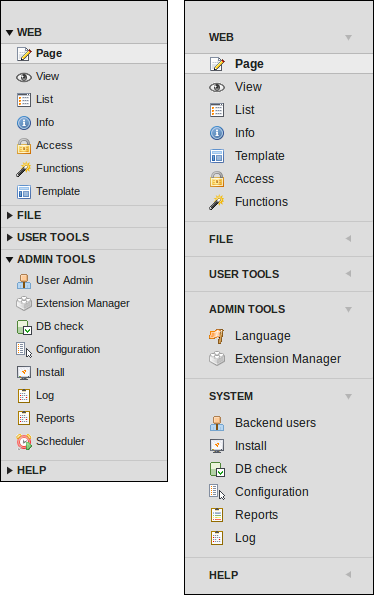
\includegraphics[width=0.6\linewidth]{Images/BackendChanges/VisualAppearance.png}
			\end{figure}
		\end{column}

	\end{columns}

\end{frame}

% ------------------------------------------------------------------------------
% Visual Appearance
% ------------------------------------------------------------------------------

\begin{frame}[fragile]
	\frametitle{Backend Changes}
	\framesubtitle{Visual Appearance}

	\begin{columns}[T]

		\begin{column}{.5\textwidth}

			\begin{itemize}
				\item Modules in left-hand-side column restructured
				\item Module "ADMINTOOLS" divided into two parts:

					\begin{itemize}
						\item \textbf{ADMINTOOLS} ("Languages" and "Extension Manager")
						\item \textbf{SYSTEM} (low-level tools, which do not show the page tree column)
					\end{itemize}

				\item Module "TypoScript Help" removed (obsolete)

			\end{itemize}

		\end{column}

		\begin{column}{.5\textwidth}
			\begin{figure}\vspace*{-0.4cm}
				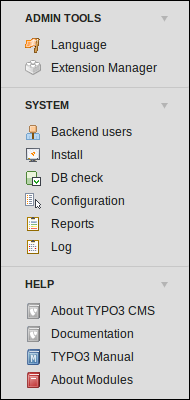
\includegraphics[width=0.35\linewidth]{Images/BackendChanges/AdminTools.png}
			\end{figure}
		\end{column}

	\end{columns}

\end{frame}

% ------------------------------------------------------------------------------
% Visual Appearance
% ------------------------------------------------------------------------------
% http://forge.typo3.org/issues/36017

\begin{frame}[fragile]
	\frametitle{Backend Changes}
	\framesubtitle{Visual Appearance}

	\begin{itemize}
		\item \texttt{<h1>}-headlines in main area use TYPO3 font "Share" consistantly
	\end{itemize}

	\begin{figure}
		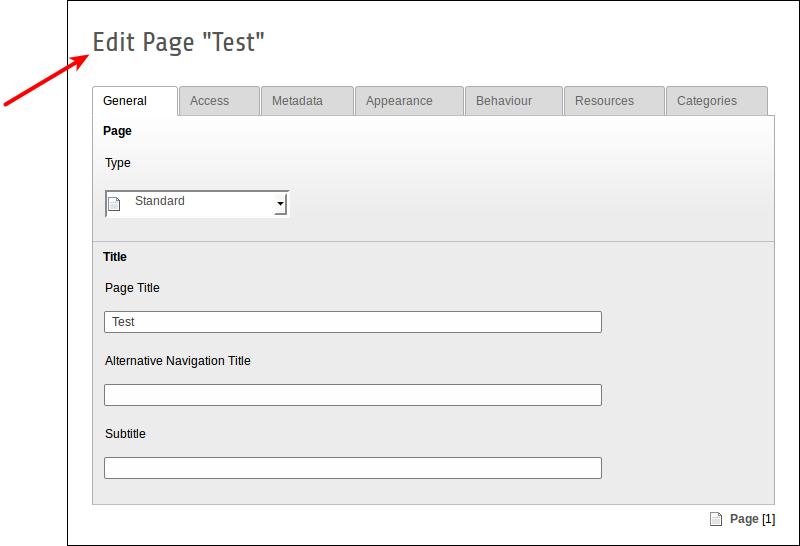
\includegraphics[width=0.6\linewidth]{Images/BackendChanges/ConsistantFont.png}
	\end{figure}

\end{frame}

% ------------------------------------------------------------------------------
% Visual Appearance
% ------------------------------------------------------------------------------
% http://forge.typo3.org/issues/41631

\begin{frame}[fragile]
	\frametitle{Backend Changes}
	\framesubtitle{Visual Appearance}

	\begin{itemize}
		\item Module "Reports" shows new icon
	\end{itemize}

	\begin{figure}
		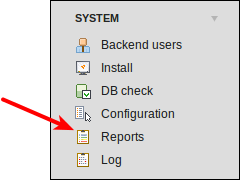
\includegraphics[width=0.35\linewidth]{Images/BackendChanges/ModuleReportsIcon.png}
	\end{figure}

\end{frame}

% ------------------------------------------------------------------------------
% Drag&Drop File Upload in Filelist (FAL)
% ------------------------------------------------------------------------------
% http://forge.typo3.org/issues/47005

\begin{frame}[fragile]
	\frametitle{Backend Changes}
	\framesubtitle{Drag\&Drop File Upload (1)}

	\begin{itemize}
		\item HTML5 Drag\&Drop file upload functionality implemented in filelist

	\end{itemize}

	\begin{figure}
		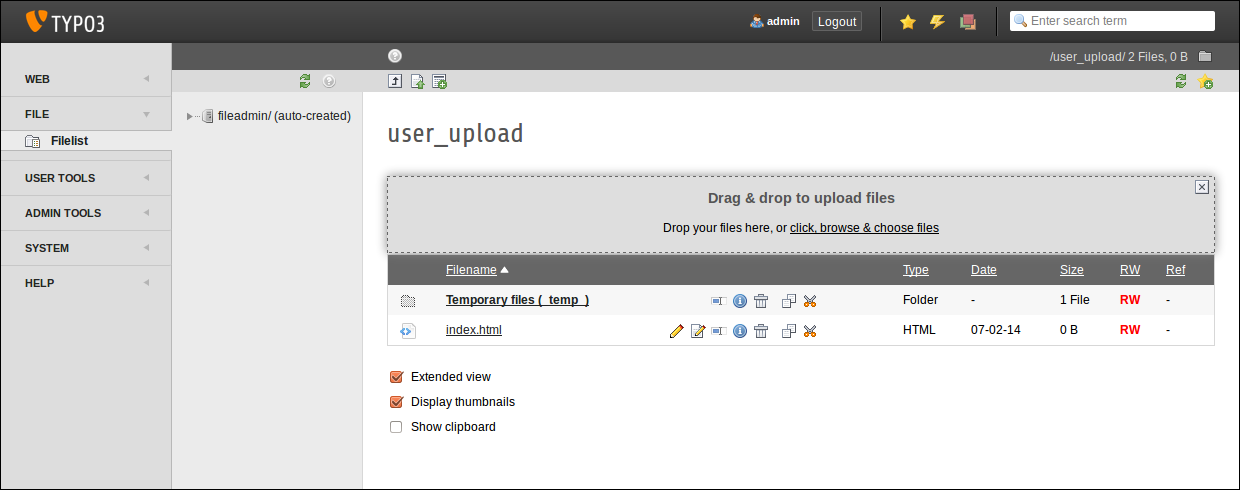
\includegraphics[width=0.95\linewidth]{Images/BackendChanges/DragDropFileUpload.png}
	\end{figure}

\end{frame}

% ------------------------------------------------------------------------------
% Drag&Drop File Upload Via Content Elements
% (slide added in March 2014)
% ------------------------------------------------------------------------------

\begin{frame}[fragile]
	\frametitle{Backend Changes}
	\framesubtitle{Drag\&Drop File Upload (2)}

	\begin{itemize}
		\item ...and via content elements (button: "Select \& upload files")

	\end{itemize}

	\begin{figure}
		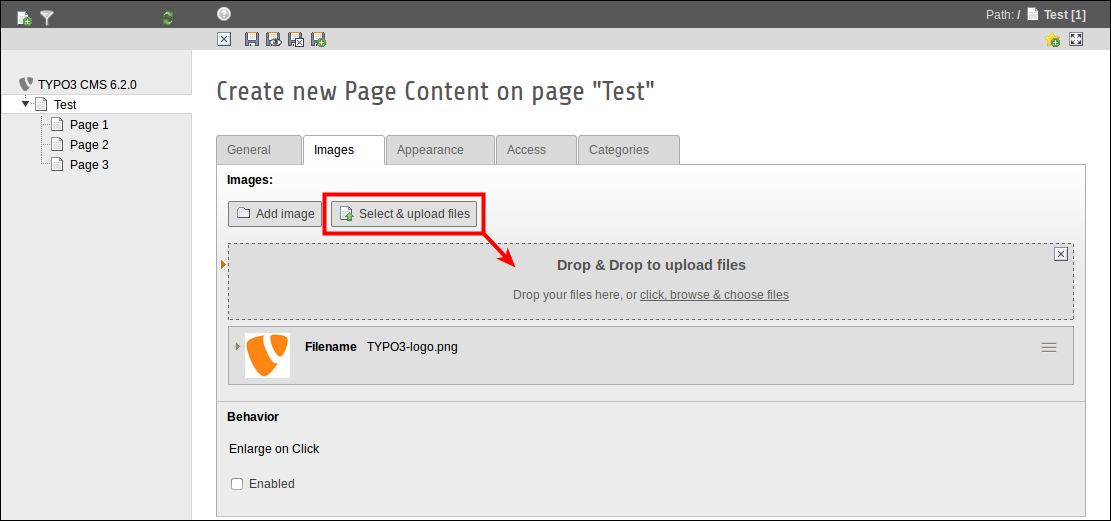
\includegraphics[width=0.95\linewidth]{Images/BackendChanges/SelectAndUploadFiles.png}
	\end{figure}

\end{frame}

% ------------------------------------------------------------------------------
% Backend Users
% ------------------------------------------------------------------------------
% http://forge.typo3.org/issues/43053

\begin{frame}[fragile]
	\frametitle{Backend Changes}
	\framesubtitle{Usability: Backend User List}

	\begin{itemize}
		\item Username and real name is shown (first column in list view)
		\item Click on (user)name links to edit user record
		\item Delete button added to list view

	\end{itemize}

	\begin{figure}
		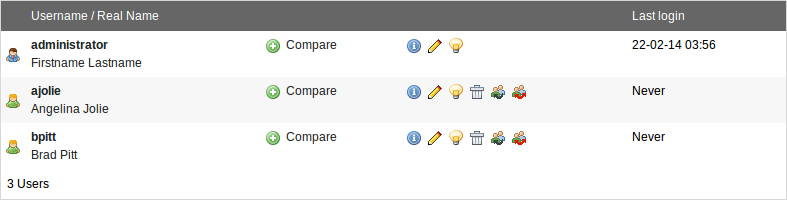
\includegraphics[width=0.95\linewidth]{Images/BackendChanges/BackendUserList.png}
	\end{figure}

\end{frame}

% ------------------------------------------------------------------------------
% Live Search
% ------------------------------------------------------------------------------
% http://forge.typo3.org/issues/35358

\begin{frame}[fragile]
	\frametitle{Backend Changes}
	\framesubtitle{Live Search}

	\begin{itemize}
		\item Tooltip shows UID as well as PID in "livesearch"
		\item When, after a search, the edit form is closed again, the list view of the page is shown (not an empty page)
	\end{itemize}

	\begin{figure}
		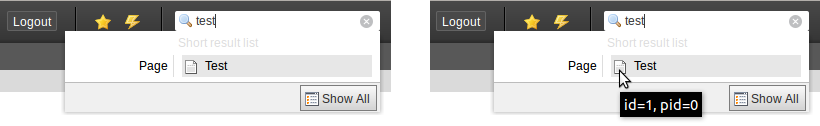
\includegraphics[width=0.8\linewidth]{Images/BackendChanges/LiveSearchTooltip.png}
	\end{figure}

\end{frame}

% ------------------------------------------------------------------------------
% Live Search
% ------------------------------------------------------------------------------

\begin{frame}[fragile]
	\frametitle{Backend Changes}
	\framesubtitle{Live Search}

	\begin{itemize}
		\item In TYPO3 < 6.2, for pages, only database fields \texttt{title} and \texttt{uid} are taken into account
		\item In TYPO3 >= 6.2, field \texttt{alias} can be added to search\newline
			(requires UserTSconfig: \texttt{options.pageTree.searchInAlias = 1})
	\end{itemize}

	\begin{figure}
		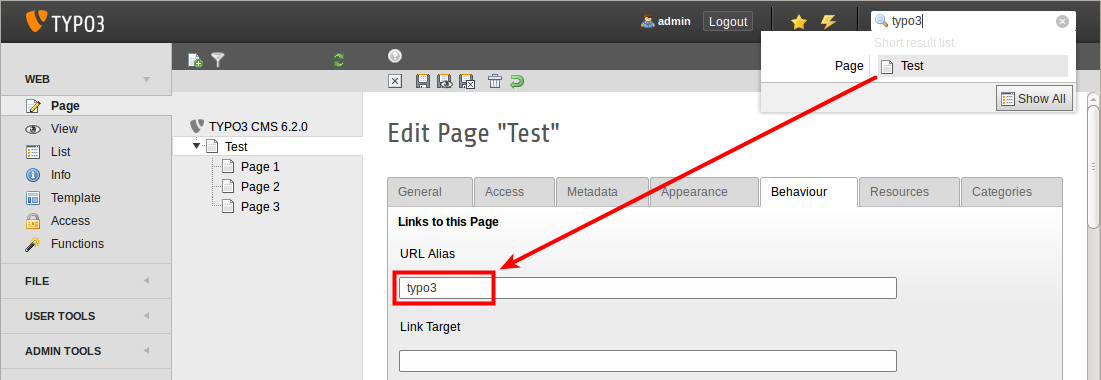
\includegraphics[width=0.95\linewidth]{Images/BackendChanges/LiveSearchInAlias.png}
	\end{figure}

\end{frame}

% ------------------------------------------------------------------------------
% File Abstraction Layer
% ------------------------------------------------------------------------------

\begin{frame}[fragile]
	\frametitle{Backend Changes}
	\framesubtitle{File Abstraction Layer}

	\begin{itemize}
		\item Title and filename are shown in FAL element header
	\end{itemize}

	\begin{figure}
		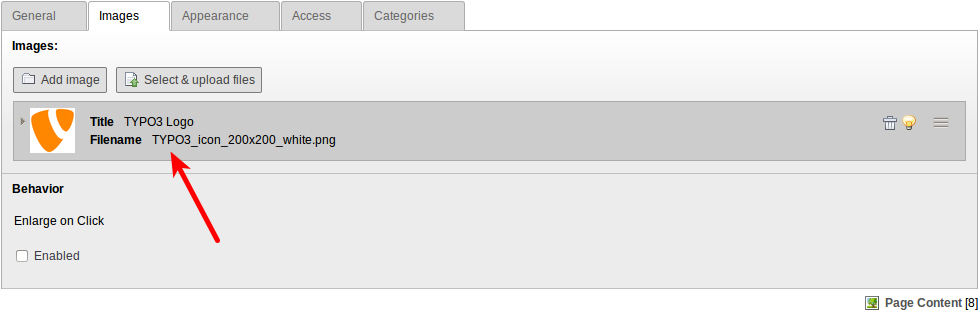
\includegraphics[width=0.95\linewidth]{Images/BackendChanges/FalTitleAndFilename.png}
	\end{figure}

\end{frame}

% ------------------------------------------------------------------------------
% File Abstraction Layer
% ------------------------------------------------------------------------------

\begin{frame}[fragile]
	\frametitle{Backend Changes}
	\framesubtitle{File Abstraction Layer (EXT:filemetadata)}

	\begin{itemize}
		\item System extension "filemetadata" add tabs to show meta data\newline
			\small(extension is shipped with the core, but not installed by default)\normalsize
	\end{itemize}

	\begin{figure}
		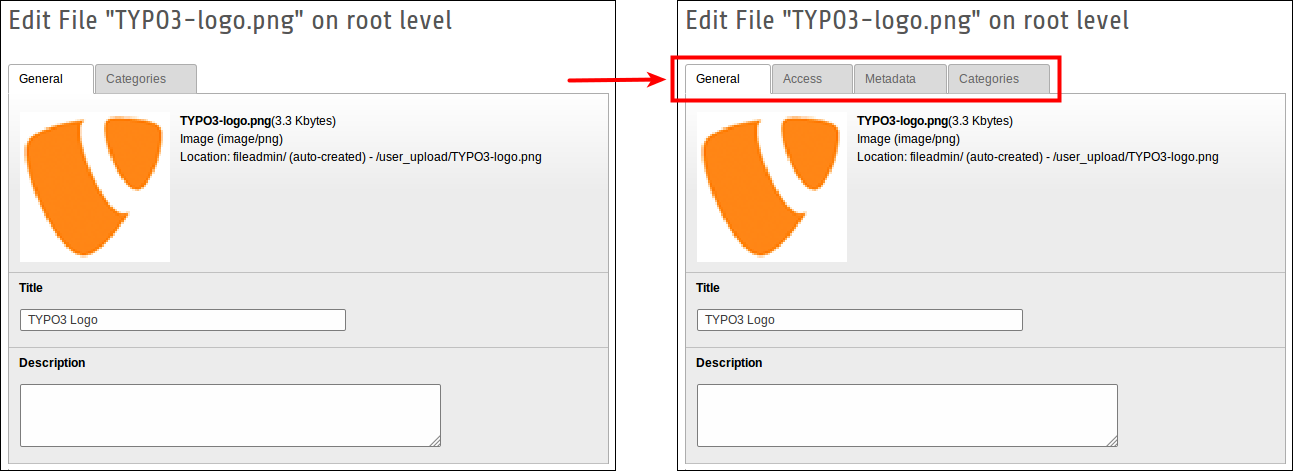
\includegraphics[width=0.95\linewidth]{Images/BackendChanges/FileMetaDataTabs.png}
	\end{figure}

\end{frame}

% ------------------------------------------------------------------------------
% File Abstraction Layer
% ------------------------------------------------------------------------------

\begin{frame}[fragile]
	\frametitle{Backend Changes}
	\framesubtitle{File Abstraction Layer (EXT:filemetadata)}

	\begin{figure}
		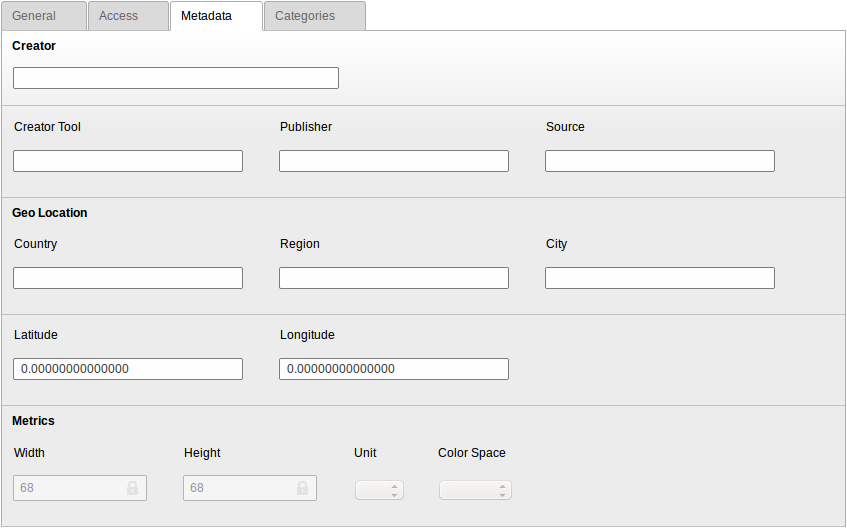
\includegraphics[width=0.8\linewidth]{Images/BackendChanges/FileMetaData.png}
	\end{figure}

\end{frame}

% ------------------------------------------------------------------------------
% File Abstraction Layer
% ------------------------------------------------------------------------------

\begin{frame}[fragile]
	\frametitle{Backend Changes}
	\framesubtitle{File Abstraction Layer}

	\begin{itemize}
		\item It is now possible to translate FAL meta data into frontend languages
	\end{itemize}

	\begin{figure}
		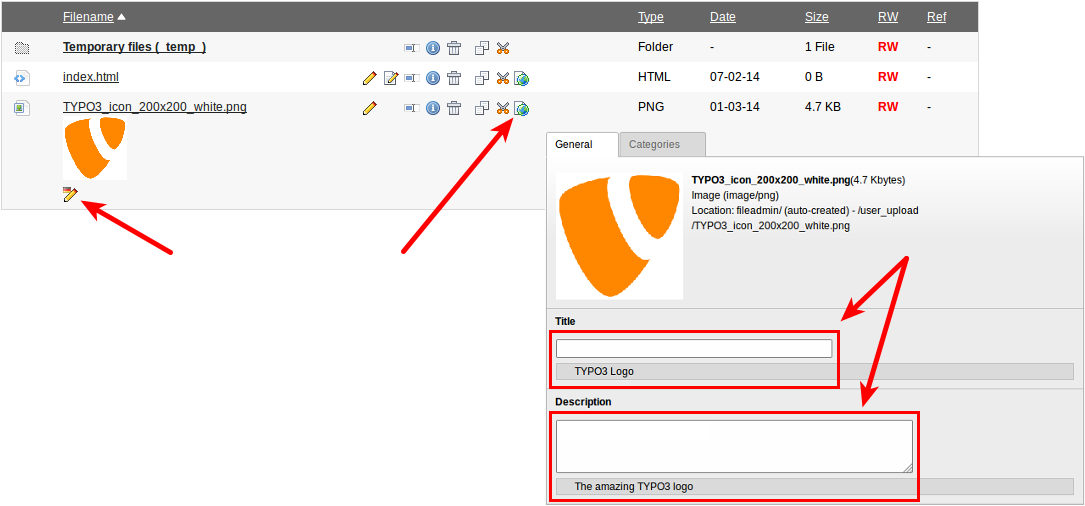
\includegraphics[width=0.95\linewidth]{Images/BackendChanges/FalTranslateMetaData.png}
	\end{figure}

\end{frame}

% ------------------------------------------------------------------------------
% Module: Documentation
% ------------------------------------------------------------------------------

\begin{frame}[fragile]
	\frametitle{Backend Changes}
	\framesubtitle{Module: Documentation}

	\begin{columns}[T]

		\begin{column}{.5\textwidth}
			\begin{itemize}
				\item Module "Documentation" allows BE users to download and view manuals
				\item New TYPO3 installations load this module by default
				\item Function "Download Documentation" downloads manuals (see illustration)
				\item Use the Extension Manager to load "Documentation" in an updated TYPO3 installation
			\end{itemize}
		\end{column}

		\begin{column}{.5\textwidth}
			\begin{figure}\vspace*{-0.4cm}
				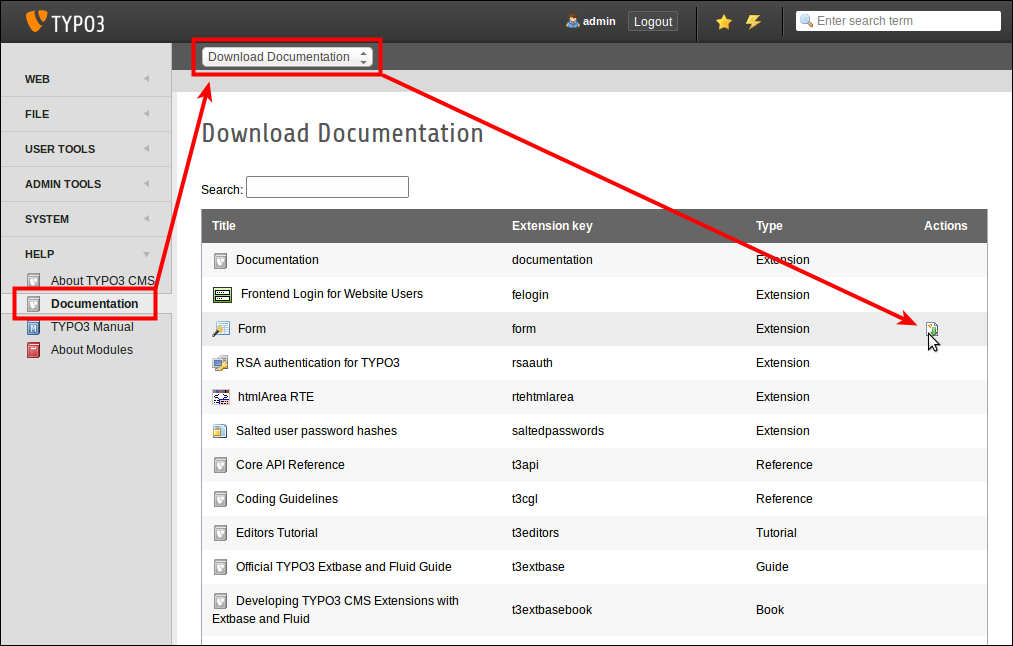
\includegraphics[width=1\linewidth]{Images/BackendChanges/DownloadDocumentation.png}
			\end{figure}
		\end{column}

	\end{columns}

\end{frame}

% ------------------------------------------------------------------------------
% Module: Documentation
% ------------------------------------------------------------------------------

\begin{frame}[fragile]
	\frametitle{Backend Changes}
	\framesubtitle{Module: Documentation}

	\begin{itemize}
		\item Function "Show Documentation" displays downloaded manuals
	\end{itemize}

	\begin{figure}
		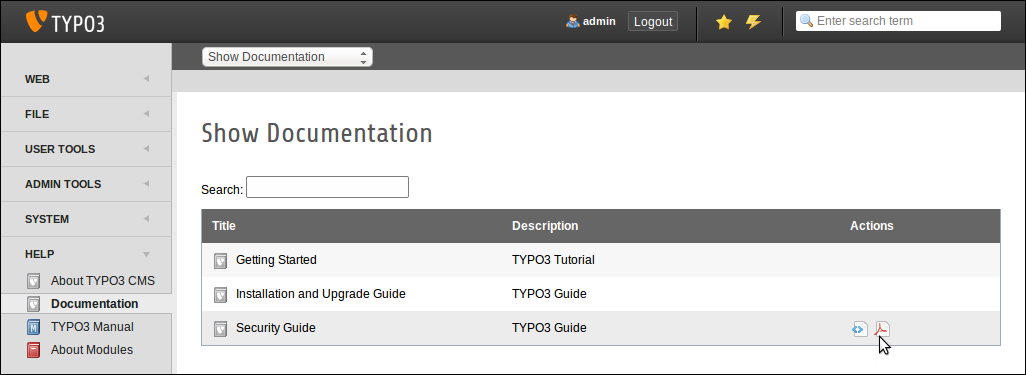
\includegraphics[width=0.95\linewidth]{Images/BackendChanges/ShowDocumentation.png}
	\end{figure}

\end{frame}

% ------------------------------------------------------------------------------
% Removed: TypoScript Help
% ------------------------------------------------------------------------------
% http://forge.typo3.org/issues/47931

\begin{frame}[fragile]
	\frametitle{Backend Changes}
	\framesubtitle{Removed: TypoScript Help}

 	\begin{itemize}
		\item EXT:tsconfig\_help ("TSconfig Quick Reference") removed\newline
			\small(outdated information and not maintained since TYPO3 CMS 4.1)
	\end{itemize}

	\begin{figure}
		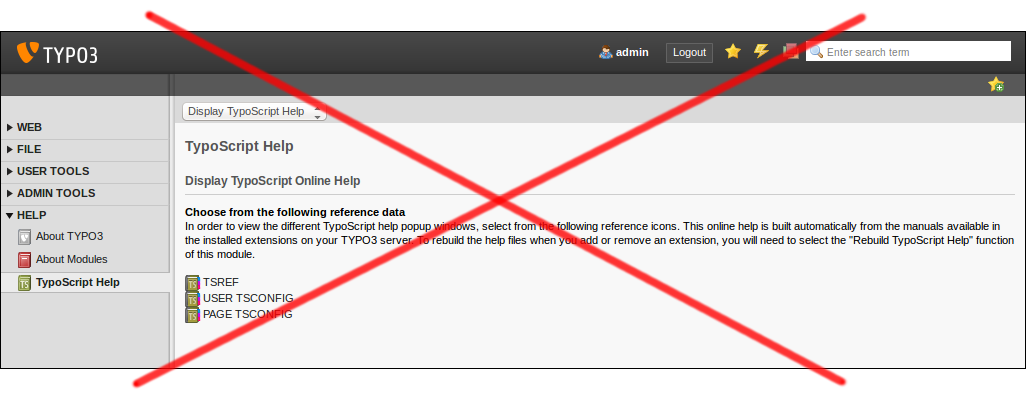
\includegraphics[width=0.95\linewidth]{Images/BackendChanges/TypoScriptHelpRemovedCrossed.png}
	\end{figure}

\end{frame}


% ------------------------------------------------------------------------------
% Scheduler
% ------------------------------------------------------------------------------

\begin{frame}[fragile]
	\frametitle{Backend Changes}
	\framesubtitle{Scheduler}

	\begin{itemize}
		\item Delete scheduler task in edit view\newline
			\small(in TYPO3 < 6.2, delete function was available in the list view only)\normalsize
	\end{itemize}

	\begin{figure}
		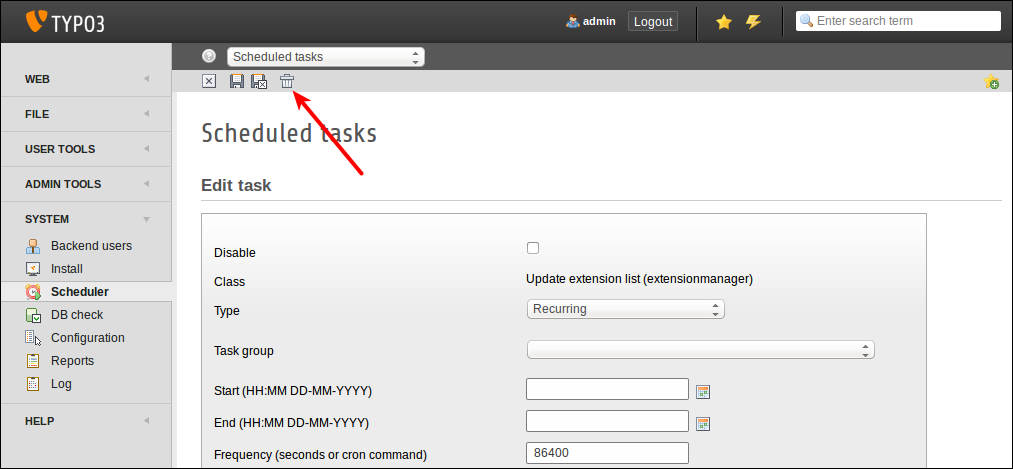
\includegraphics[width=0.95\linewidth]{Images/BackendChanges/DeleteSchedulerTaskInEditView.png}
	\end{figure}

\end{frame}

% ------------------------------------------------------------------------------
% Scheduler
% ------------------------------------------------------------------------------

\begin{frame}[fragile]
	\frametitle{Backend Changes}
	\framesubtitle{Scheduler}

	\begin{itemize}
		\item Description can be assigned to scheduler tasks and shown as subheaders in list view, or as tooltips (see next slide)
	\end{itemize}

	\begin{figure}
		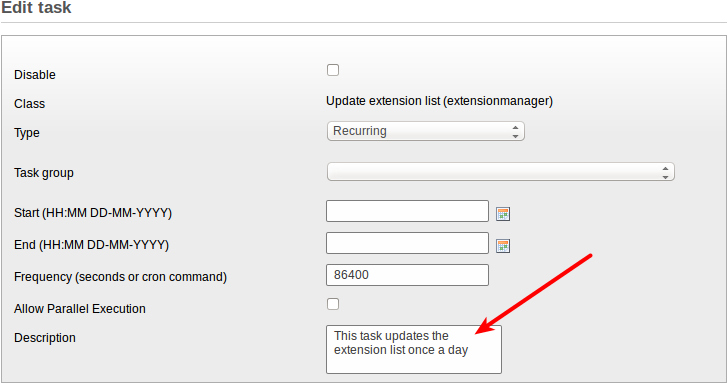
\includegraphics[width=0.7\linewidth]{Images/BackendChanges/SchedulerTaskDescription.png}
	\end{figure}

\end{frame}

% ------------------------------------------------------------------------------
% Scheduler
% ------------------------------------------------------------------------------

\begin{frame}[fragile]
	\frametitle{Backend Changes}
	\framesubtitle{Scheduler}

	\begin{itemize}
		\item Task description as subheader\newline
			\small(this features needs to be activated in extension configuration)\normalsize
	\end{itemize}

	\begin{figure}
		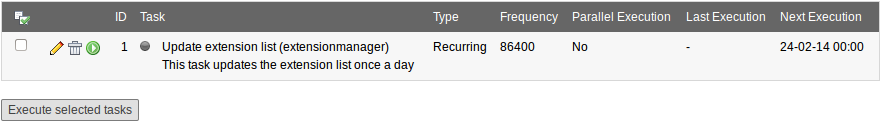
\includegraphics[width=0.95\linewidth]{Images/BackendChanges/SchedulerTaskDescriptionAsSubheader.png}
	\end{figure}

	\begin{itemize}
		\item Task description as tooltip ("hover")
	\end{itemize}

	\begin{figure}
		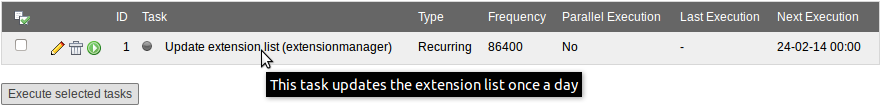
\includegraphics[width=0.95\linewidth]{Images/BackendChanges/SchedulerTaskDescriptionAsTooltip.png}
	\end{figure}

\end{frame}

% ------------------------------------------------------------------------------
% Scheduler
% ------------------------------------------------------------------------------

\begin{frame}[fragile]
	\frametitle{Backend Changes}
	\framesubtitle{Scheduler}

	\begin{itemize}
		\item It is now possible to group scheduler tasks
		\item Add "scheduler task group" records to root page (UID: 0)\newline
			and select group in the task
	\end{itemize}

	\begin{figure}
		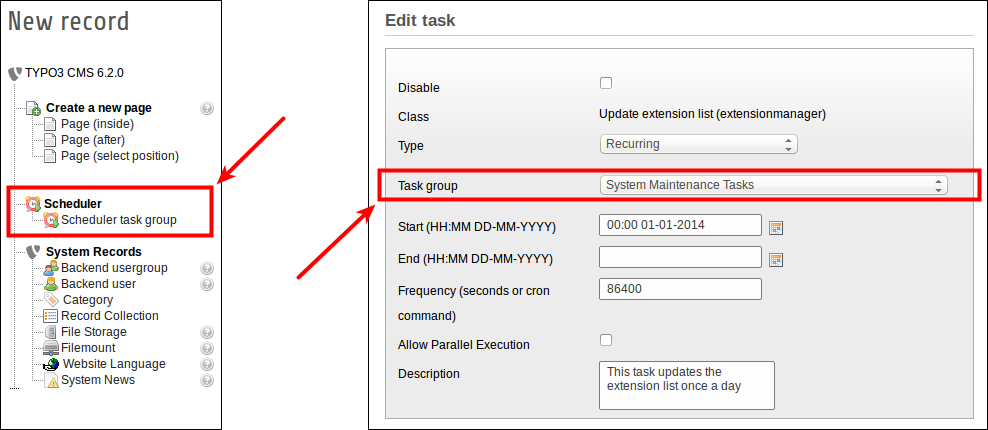
\includegraphics[width=0.85\linewidth]{Images/BackendChanges/SchedulerTaskGroup.png}
	\end{figure}

\end{frame}

% ------------------------------------------------------------------------------
% System Extension: Form
% ------------------------------------------------------------------------------
% http://forge.typo3.org/issues/38094

\begin{frame}[fragile]
	\frametitle{Backend Changes}
	\framesubtitle{System Extension: Form}

	\begin{columns}[T]

		\begin{column}{.5\textwidth}
			\begin{itemize}
				\item New post-processor for cObject FORM: \textbf{redirect}\newline
					(redirect after form submission)
				\item Value is parsed by \texttt{typolink} (TypoScript function),\newline
					which means, value can be a page ID or a URL
			\end{itemize}
		\end{column}

		\begin{column}{.5\textwidth}
			\begin{figure}\vspace*{-0.4cm}
				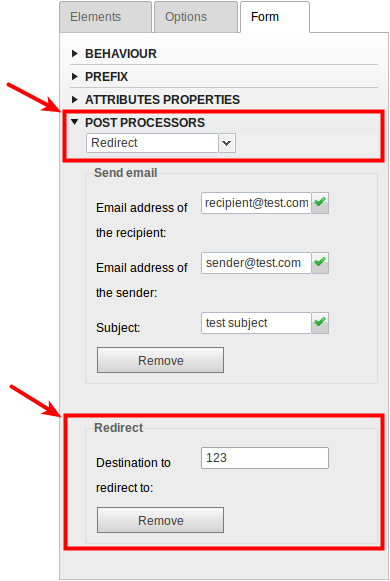
\includegraphics[width=0.65\linewidth]{Images/BackendChanges/FormRedirectPostProcessor.png}
			\end{figure}
		\end{column}

	\end{columns}

\end{frame}

% ------------------------------------------------------------------------------
% Module: List
% ------------------------------------------------------------------------------
% http://forge.typo3.org/issues/49810

\begin{frame}[fragile]
	\frametitle{Backend Changes}
	\framesubtitle{List Module}

	\begin{itemize}
		\item Additional columns "UID" and "PID" in list view for non-admins
	\end{itemize}

	\begin{figure}
		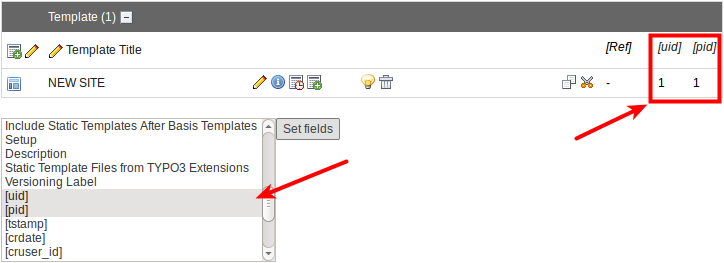
\includegraphics[width=0.95\linewidth]{Images/BackendChanges/AdditionalColumnsInListModule.png}
	\end{figure}

\end{frame}

% ------------------------------------------------------------------------------
% File Abstraction Layer
% ------------------------------------------------------------------------------
% http://forge.typo3.org/issues/50827
% http://forge.typo3.org/issues/51097

\begin{frame}[fragile]
	\frametitle{Backend Changes}
	\framesubtitle{File Abstraction Layer}

	\begin{itemize}
		\item If indexer detects a missing file, a message is shown and a flag in the database record is set
		\item Module "Reports" also lists this as an issue
		\item When file re-appears, message and flag are reset
	\end{itemize}

	\begin{columns}[T]

		\begin{column}{.5\textwidth}
			\begin{figure}
				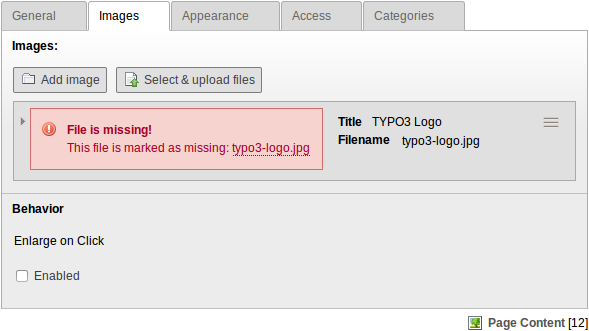
\includegraphics[width=0.95\linewidth]{Images/BackendChanges/FalMissingFileContentElement.png}
			\end{figure}
		\end{column}

		\begin{column}{.5\textwidth}
			\begin{figure}
				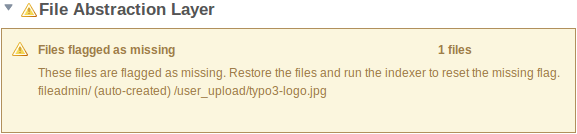
\includegraphics[width=0.95\linewidth]{Images/BackendChanges/FalMissingFileReportsModule.png}
			\end{figure}
		\end{column}

	\end{columns}

\end{frame}

% ------------------------------------------------------------------------------
% Menu/Sitemap: Category-based Menus
% ------------------------------------------------------------------------------
% http://forge.typo3.org/issues/51161

\begin{frame}[fragile]
	\frametitle{Backend Changes}
	\framesubtitle{Category-based Menus (1)}

	\begin{itemize}
		\item Content element "Menu/Sitemap" can create a menu, based on categories
	\end{itemize}

	\begin{figure}
		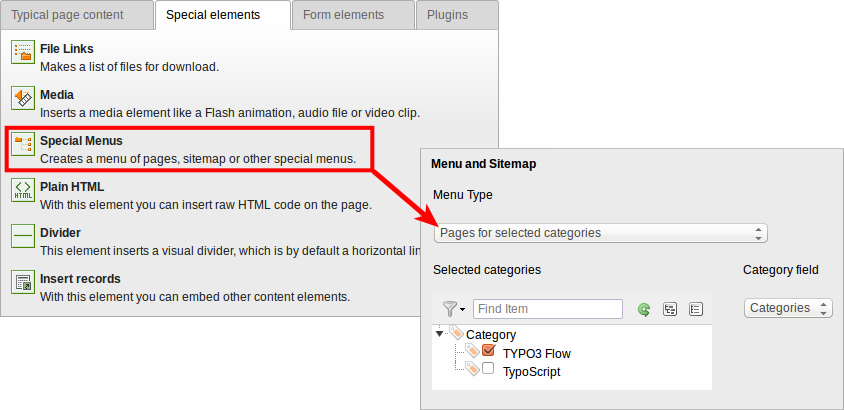
\includegraphics[width=0.8\linewidth]{Images/BackendChanges/CategoryBasedMenus.png}
	\end{figure}

\end{frame}

% ------------------------------------------------------------------------------
% Menu/Sitemap: Category-based Menus
% (slide added in March 2014)
% ------------------------------------------------------------------------------

\begin{frame}[fragile]
	\frametitle{Backend Changes}
	\framesubtitle{Category-based Menus (2)}

	\begin{itemize}
		\item Another new type of menu: "\underline{Content elements} for selected categories"
	\end{itemize}

	\begin{figure}
		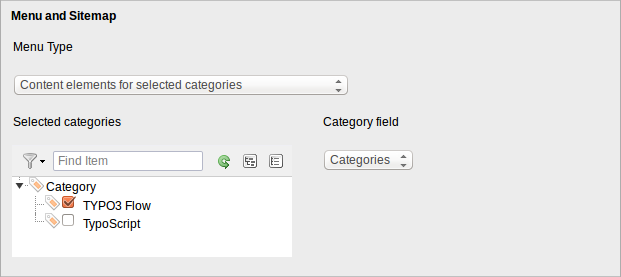
\includegraphics[width=0.6\linewidth]{Images/BackendChanges/ContentElementsForSelectedCategories.png}
	\end{figure}

\end{frame}

% ------------------------------------------------------------------------------
% Sorting Categories
% ------------------------------------------------------------------------------
% http://forge.typo3.org/issues/51590

\begin{frame}[fragile]
	\frametitle{Backend Changes}
	\framesubtitle{Sorting Categories}

 	\begin{itemize}
		\item Categories can be sorted now\newline
			\small(in TYPO3 < 6.2, categories are always sorted alphabetically)\normalsize
	\end{itemize}

	\begin{figure}
		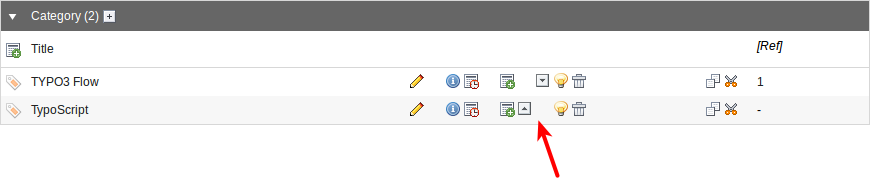
\includegraphics[width=0.95\linewidth]{Images/BackendChanges/CategorySorting.png}
	\end{figure}

\end{frame}

% ------------------------------------------------------------------------------
% Category Visibility
% ------------------------------------------------------------------------------
% http://forge.typo3.org/issues/52718

\begin{frame}[fragile]
	\frametitle{Backend Changes}
	\framesubtitle{Category Visibility}

 	\begin{itemize}
		\item Visibility of categories can be restricted for BE users/groups
	\end{itemize}

	\begin{figure}
		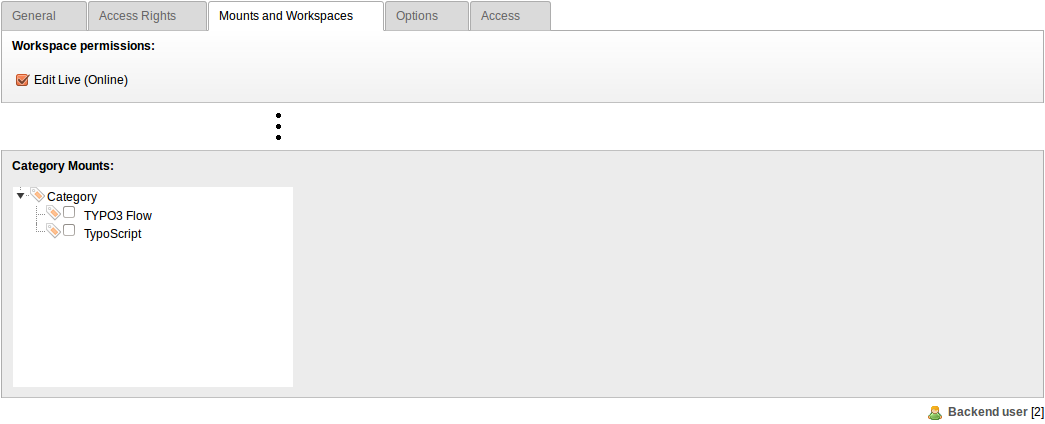
\includegraphics[width=0.95\linewidth]{Images/BackendChanges/CategoryVisibility.png}
	\end{figure}

\end{frame}

% ------------------------------------------------------------------------------
% "New Content" icon always visible
% ------------------------------------------------------------------------------
% http://forge.typo3.org/issues/48938
% http://forge.typo3.org/issues/51480

\begin{frame}[fragile]
	\frametitle{Backend Changes}
	\framesubtitle{Usability}

 	\begin{itemize}
		\item Icon "new content" is always visible if the column is empty\newline
			\small(this helps editors to understand what they can do)\normalsize
	\end{itemize}

	\begin{figure}
		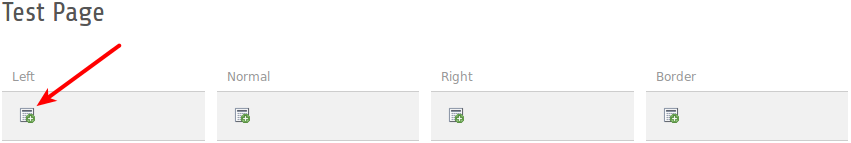
\includegraphics[width=0.95\linewidth]{Images/BackendChanges/NewContentIconAlwaysVisible.png}
	\end{figure}

\end{frame}

% ------------------------------------------------------------------------------
% Module "Functions": Hide In Menus
% ------------------------------------------------------------------------------
% http://forge.typo3.org/issues/51017

\begin{frame}[fragile]
	\frametitle{Backend Changes}
	\framesubtitle{Functions}

 	\begin{itemize}
		\item When creating multiple pages in module "functions", a new checkbox allows editors to hide these pages in menus\newline
			\small(very useful, when creating a number of pages at a time)\normalsize
	\end{itemize}

	\begin{figure}
		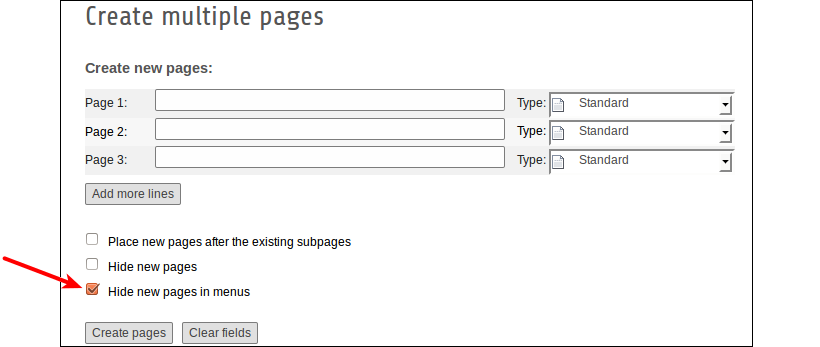
\includegraphics[width=0.85\linewidth]{Images/BackendChanges/CreateMultiplePagesHideInMenu.png}
	\end{figure}

\end{frame}

% ------------------------------------------------------------------------------
% Extension Manager: Upload Extensions
% ------------------------------------------------------------------------------
% http://forge.typo3.org/issues/51776
% http://forge.typo3.org/issues/51437

\begin{frame}[fragile]
	\frametitle{Backend Changes}
	\framesubtitle{Extension Manager}

 	\begin{itemize}
		\item Upload an extension via the "Get Extensions" function
	\end{itemize}

	\begin{figure}
		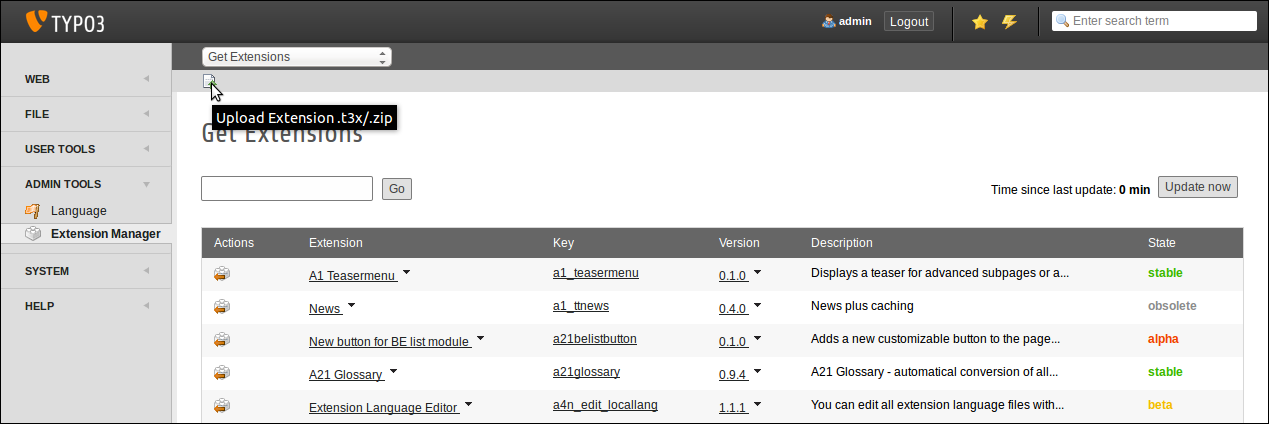
\includegraphics[width=0.95\linewidth]{Images/BackendChanges/UploadExtension.png}
	\end{figure}

\end{frame}

% ------------------------------------------------------------------------------
% Recycler
% ------------------------------------------------------------------------------
% http://forge.typo3.org/issues/52324

\begin{frame}[fragile]
	\frametitle{Backend Changes}
	\framesubtitle{Recycler}

 	\begin{itemize}
		\item Recycler records can be sorted by time stamp\newline
			\small(this helps users to decide whether to recover a specific record or not)\normalsize
	\end{itemize}

	\begin{figure}
		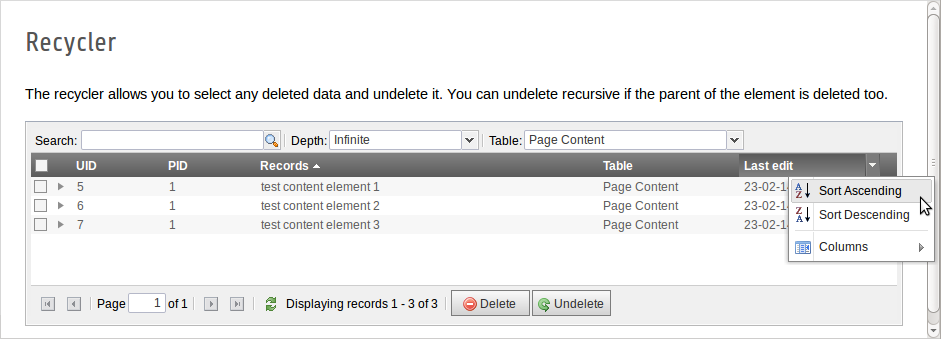
\includegraphics[width=0.95\linewidth]{Images/BackendChanges/RecyclerSortRecord.png}
	\end{figure}

\end{frame}

% ------------------------------------------------------------------------------
% File/Directory Permissions
% ------------------------------------------------------------------------------

\begin{frame}[fragile]
	\frametitle{Backend Changes}
	\framesubtitle{File/Directory Permissions}

 	\begin{itemize}
		\item Much more granular file/directory permissions for BE users/groups
			\begingroup\color{typo3red}\textbf{(1)}\endgroup
		\item This is possible since TYPO3 6.0, but only via UserTSconfig
			\begingroup\color{typo3red}\textbf{(2)}\endgroup
	\end{itemize}

	\begin{figure}
		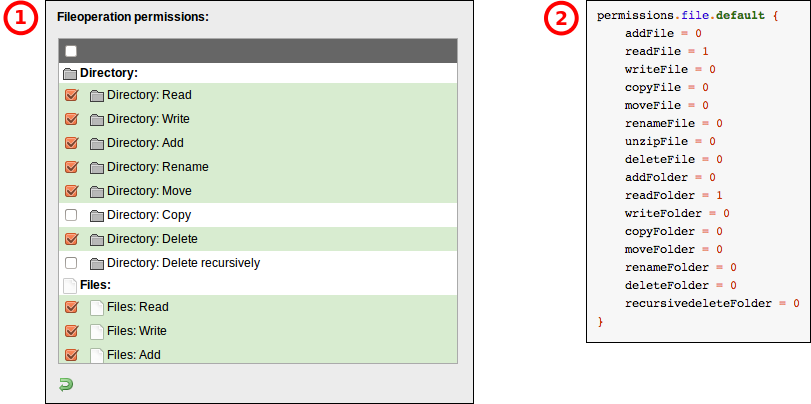
\includegraphics[width=0.75\linewidth]{Images/BackendChanges/FileAndDirectoryPermissions.png}
	\end{figure}

\end{frame}

% ------------------------------------------------------------------------------
% OpenID
% ------------------------------------------------------------------------------

\begin{frame}[fragile]
	\frametitle{Backend Changes}
	\framesubtitle{OpenID (1)}

 	\begin{itemize}
		\item OpenID for BE user authentication can be configured by using a wizard
		\item EXT:openid (system extension) is required for this feature
	\end{itemize}

	\begin{figure}
		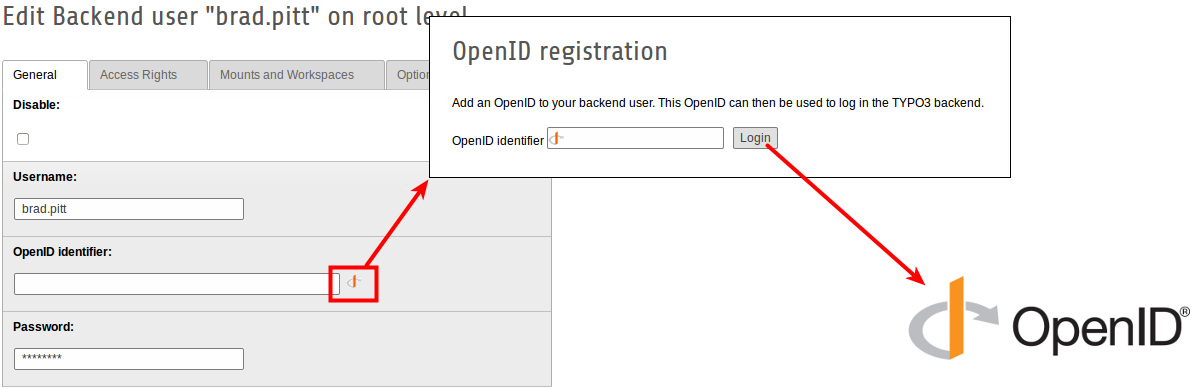
\includegraphics[width=0.95\linewidth]{Images/BackendChanges/OpenIdWizard.png}
	\end{figure}

\end{frame}

% ------------------------------------------------------------------------------
% OpenID
% ------------------------------------------------------------------------------

\begin{frame}[fragile]
	\frametitle{Backend Changes}
	\framesubtitle{OpenID (2)}

 	\begin{itemize}
		\item OpenID for BE user authentication can be configured by using a wizard
		\item EXT:openid (system extension) is required for this feature
	\end{itemize}

	\begin{figure}
		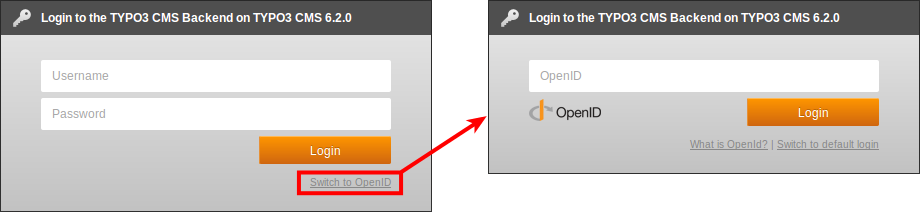
\includegraphics[width=0.8\linewidth]{Images/BackendChanges/OpenIdLogin.png}
	\end{figure}

 	\begin{itemize}
		\item Further details about OpenID:\newline
			\small\url{http://openid.net}\normalsize
	\end{itemize}

\end{frame}

% ------------------------------------------------------------------------------
% Workspaces
% ------------------------------------------------------------------------------
% http://forge.typo3.org/issues/50223
% http://forge.typo3.org/issues/50224

\begin{frame}[fragile]
	\frametitle{Backend Changes}
	\framesubtitle{Workspaces}

 	\begin{itemize}
		\item Editors/users can define who to notify, without limiting this on the system level
		\item Tab "All" is now visible to \underline{all} users
	\end{itemize}

	\begin{figure}
		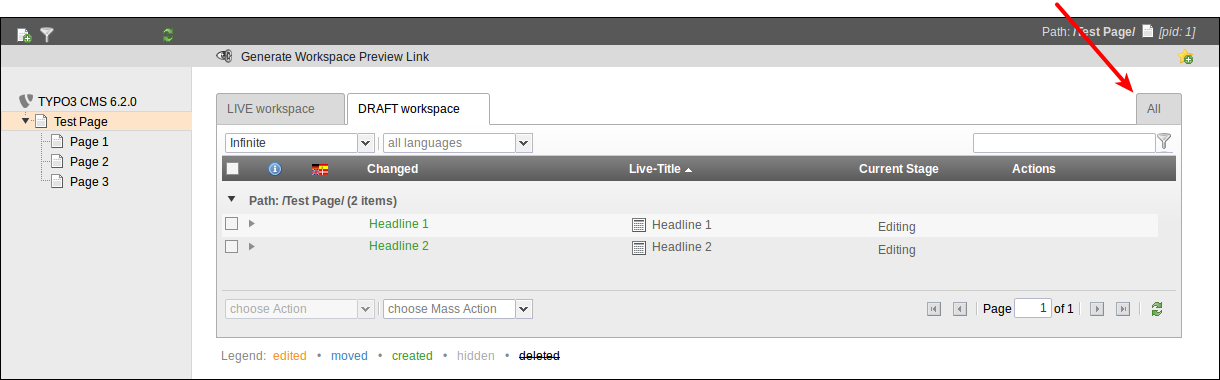
\includegraphics[width=0.95\linewidth]{Images/BackendChanges/WorkspacesTabAll.png}
	\end{figure}

\end{frame}

% ------------------------------------------------------------------------------

